%%=============================================================================
%% Methodologie
%%=============================================================================

\chapter{Resultaat van de Enquête}
\label{ch:resultaten_vragen}

In totaal vulden in de periode tussen 8 april en 7 mei 404 studenten, verspreid over de Hogeschool Gent in België en de Haagse Hogeschool in Nederland, de enquête in. Het nam de student gemiddeld 7 minuten en 52 seconden om de enquête in te vullen.

\begin{figure}
	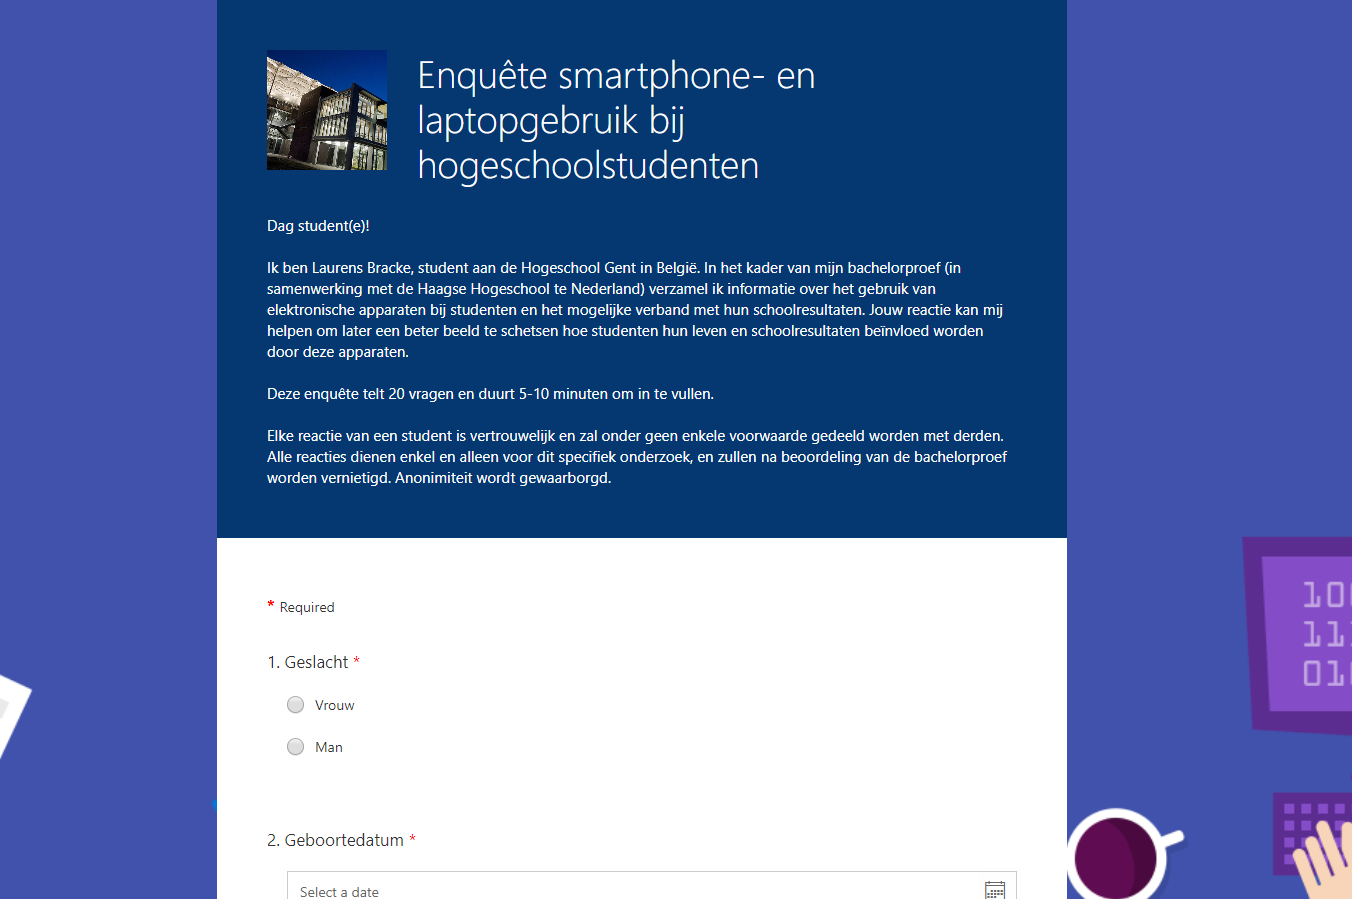
\includegraphics[width=\textwidth]
	{img/vragen-enquete.png}
	\caption{Vragen enquête voor studenten Haagse Hogeschool en HoGent }
	\label{fig:vragen-enquete}
\end{figure}

In figuur \ref{fig:vragen-enquete} vindt u een screenshot terug van de online vragenlijst over hun gebruik van smartphones, laptops en hun laatste studieresultaten. 

De vragen kan u terugvinden in bijlage \ref{ch:vragenlijst}.

De resultaten van deze test kan u terugvinden via volgende weblink (in Excel-formaat): \url{https://1drv.ms/f/s!AnudQT05fzZSlx83i8B1_PG0OKxa} 

Door middel van het gebruik van een steekproefcalculator (bijvoorbeeld \url{nl.checkmarket.com/steekproefcalculator}) en het cijfermateriaal uit de literatuurstudie kunnen we vaststellen dat het aantal resultaten dat we nodig hadden voor significante resultaten te bekomen te weinig is voor dit onderzoek. Indien we zowel in Nederland als in België nog 100 extra studenten konden bereiken in deze periode, konden we mogelijks spreken van een significant onderzoek dat de volledige populatie benadert met een betrouwbaarheidsinterval van 95 procent. De Vlaamse resultaten mogen wel significant genoemd worden als we rekenen met een betrouwbaarheidsinterval van 90 procent. Onze resultaten zijn wel nog steeds een goede indicatie van de onderzochte groepen. Volgens net vernoemde site kunnen we stellen dat de bekomen resultaten moeten bekeken worden met een foutmarge van 7,51 procent voor Nederland en een foutmarge van 6,16 voor België. We gaan hier uit dat van alle verzonden invitaties via Facebook, e-mail of mondelinge communicatie 15 à 20 procent geantwoord hebben (Checkmarket.com geeft aan dat de kans dat iemand een antwoord geeft op een online enquête ongeveer 20 procent is, hoewel ze zelf aangeven dat dit een zeer positieve en rooskleurige inschatting is).

Om deze resultaten te onderzoeken, is een tabel gemaakt die bestaat uit 3 kolommen: de eerste kolom vat de resultaten van alle 404 antwoorden samen, de tweede kolom is een samenvatting van de resultaten van studenten die minder of evenveel tijd spenderen achter hun smartphone of laptop per dag dan het gemiddelde waar de derde kolom die studenten zal groeperen die qua gespendeerde tijd achter hun devices over het gemiddelde scoren. In tabel \ref{results} ziet u hiervan de uitkomst.

Aan de hand van deze tabel krijgen we al een goed beeld over onze onderzochte studenten en de procentuele verdeling van de student bij elke vraag.

\begin{landscape}
	\begin{longtable}[c]{r|cccccc|}
		\cline{2-7}
		\multicolumn{1}{l|}{} & \multicolumn{2}{c|}{Alle studenten} & \multicolumn{2}{c|}{Deelmonster A} & \multicolumn{2}{c|}{Deelmonster B} \\ \cline{2-7} 
		\endfirsthead
		%
		\multicolumn{7}{c}%
		{{\bfseries }} \\
		\cline{2-7}
		\multicolumn{1}{l|}{} & \multicolumn{2}{c|}{Alle studenten} & \multicolumn{2}{c|}{Deelmonster A} & \multicolumn{2}{c|}{Deelmonster B} \\ \cline{2-7} 
		\endhead
		%
		\hline
		\endfoot
		%
		\endlastfoot
		%
		\multicolumn{1}{l|}{} & \multicolumn{2}{c|}{Aantal = 404} & \multicolumn{2}{c|}{Aantal = 228} & \multicolumn{2}{c|}{Aantal = 176} \\ \cline{2-7} 
		\multicolumn{1}{l|}{} & \multicolumn{2}{c|}{\begin{tabular}[c]{@{}c@{}}Gemiddeld aantal uur \\ per dag achter \\ smartphone of laptop\\ is gelijk aan 7,54\end{tabular}} & \multicolumn{2}{c|}{\begin{tabular}[c]{@{}c@{}}Gemiddeld aantal uur \\ per dag achter \\ smartphone of laptop \\ is lager of gelijk aan 7,54\end{tabular}} & \multicolumn{2}{c|}{\begin{tabular}[c]{@{}c@{}}Gemiddeld aantal uur \\ per dag achter \\ smartphone of laptop \\ is groter dan 7,54\end{tabular}} \\ \cline{2-7} 
		\multicolumn{1}{l|}{} & \multicolumn{1}{c|}{\begin{tabular}[c]{@{}c@{}}Absolute\\ waarden\end{tabular}} & \multicolumn{1}{c|}{\begin{tabular}[c]{@{}c@{}}Relatieve\\ waarden\end{tabular}} & \multicolumn{1}{c|}{\begin{tabular}[c]{@{}c@{}}Absolute\\ waarden\end{tabular}} & \multicolumn{1}{c|}{\begin{tabular}[c]{@{}c@{}}Relatieve\\ waarden\end{tabular}} & \multicolumn{1}{c|}{\begin{tabular}[c]{@{}c@{}}Absolute\\ waarden\end{tabular}} & \begin{tabular}[c]{@{}c@{}}Relatieve\\ waarden\end{tabular} \\ \hline
		\multicolumn{1}{|l|}{\textbf{Geslacht}} &  &  &  &  &  &  \\
		\multicolumn{1}{|r|}{\textit{Man}} & 170 & 42,08\% & 81 & 35,53\% & 89 & 50,57\% \\
		\multicolumn{1}{|r|}{\textit{Vrouw}} & 234 & 57,92\% & 147 & 64,47\% & 87 & 49,43\% \\ \hline
		\multicolumn{1}{|l|}{\textbf{Relatiestatus}} &  &  &  &  &  &  \\
		\multicolumn{1}{|r|}{\textit{Vrijgezel}} & 246 & 60,89\% & 133 & 58,33\% & 113 & 64,20\% \\
		\multicolumn{1}{|r|}{\textit{In een relatie}} & 158 & 39,11\% & 95 & 41,67\% & 63 & 35,80\% \\ \hline
		\multicolumn{1}{|l|}{\textbf{Hogeschool}} &  &  &  &  &  &  \\
		\multicolumn{1}{|r|}{\textit{Hogeschool Gent België}} & 242 & 59,90\% & 149 & 65,35\% & 93 & 52,84\% \\
		\multicolumn{1}{|r|}{\textit{Haagse Hogeschool Nederland}} & 162 & 40,10\% & 79 & 34,65\% & 83 & 47,16\% \\ \hline
		\multicolumn{1}{|l|}{\textbf{Studierichting}} &  &  &  &  &  &  \\
		\multicolumn{1}{|r|}{\textit{Toegepaste Informatica Gent}} & 56 & 13,86\% & 18 & 7,89\% & 38 & 21,59\% \\
		\multicolumn{1}{|r|}{\textit{Bedrijfsmanagement Gent}} & 20 & 4,95\% & 15 & 6,58\% & 5 & 2,84\% \\
		\multicolumn{1}{|r|}{\textit{Sociaal Werk Gent}} & 66 & 16,34\% & 46 & 20,18\% & 20 & 11,36\% \\
		\multicolumn{1}{|r|}{\textit{Orthopedagogie Gent}} & 103 & 25,50\% & 72 & 31,58\% & 31 & 17,61\% \\
		\multicolumn{1}{|r|}{\textit{HBO-ICT Nederland}} & 108 & 26,73\% & 49 & 21,49\% & 59 & 33,52\% \\
		\multicolumn{1}{|r|}{\textit{Bedrijfskunde Nederland}} & 6 & 1,49\% & 5 & 2,19\% & 1 & 0,57\% \\
		\multicolumn{1}{|r|}{\textit{Social Work Nederland}} & 20 & 4,95\% & 10 & 4,39\% & 10 & 5,68\% \\
		\multicolumn{1}{|r|}{\textit{Pedagogiek Nederland}} & 25 & 6,19\% & 13 & 5,70\% & 12 & 6,82\% \\ \hline
		\multicolumn{1}{|l|}{\textbf{Modeltrajectjaar van student}} &  &  &  &  &  &  \\
		\multicolumn{1}{|r|}{\textit{Jaar 1}} & 138 & 34,16\% & 76 & 33,33\% & 52 & 29,55\% \\
		\multicolumn{1}{|r|}{\textit{Jaar 2}} & 114 & 28,22\% & 67 & 29,39\% & 47 & 26,70\% \\
		\multicolumn{1}{|r|}{\textit{Jaar 3}} & 125 & 30,94\% & 69 & 30,26\% & 56 & 31,82\% \\
		\multicolumn{1}{|r|}{\textit{Jaar 4 (Enkel in Nederland)}} & 27 & 6,68\% & 16 & 7,02\% & 11 & 6,25\% \\ \hline
		\multicolumn{1}{|l|}{\textbf{Aantal jaar dat student de richting volgt}} &  &  &  &  &  &  \\
		\multicolumn{1}{|r|}{\textit{1 jaar}} & 134 & 33,17\% & 77 & 33,77\% & 57 & 32,39\% \\
		\multicolumn{1}{|r|}{\textit{2 jaren}} & 111 & 27,48\% & 64 & 28,07\% & 47 & 26,70\% \\
		\multicolumn{1}{|r|}{\textit{3 jaren}} & 96 & 23,76\% & 55 & 24,12\% & 41 & 23,30\% \\
		\multicolumn{1}{|r|}{\textit{4 jaren}} & 47 & 11,63\% & 26 & 11,40\% & 21 & 11,93\% \\
		\multicolumn{1}{|r|}{\textit{5 jaren}} & 12 & 2,97\% & 5 & 2,19\% & 7 & 3,98\% \\
		\multicolumn{1}{|r|}{\textit{6 jaren of meer}} & 4 & 0,99\% & 1 & 0,44\% & 3 & 1,70\% \\ \hline
		\multicolumn{1}{|l|}{\textbf{Verblijfplaats tijdens schooljaar}} &  &  &  &  &  &  \\
		\multicolumn{1}{|r|}{\textit{Thuis}} & 298 & 73,76\% & 175 & 76,75\% & 123 & 69,89\% \\
		\multicolumn{1}{|r|}{\textit{Studentenkamer / Kot}} & 95 & 23,51\% & 48 & 21,05\% & 47 & 26,70\% \\
		\multicolumn{1}{|r|}{\textit{Andere opties}} & 11 & 2,72\% & 5 & 2,19\% & 6 & 3,41\% \\ \hline
		\multicolumn{1}{|l|}{\textbf{IT-Kennis van de ouders}} &  &  &  &  &  &  \\
		\multicolumn{1}{|r|}{\textit{Geen}} & 58 & 14,36\% & 32 & 14,04\% & 26 & 14,77\% \\
		\multicolumn{1}{|r|}{\textit{Weinig}} & 97 & 24,01\% & 55 & 24,12\% & 42 & 23,86\% \\
		\multicolumn{1}{|r|}{\textit{Voldoende}} & 144 & 35,64\% & 80 & 35,09\% & 64 & 36,36\% \\
		\multicolumn{1}{|r|}{\textit{Goed}} & 86 & 21,29\% & 50 & 21,93\% & 47 & 26,70\% \\
		\multicolumn{1}{|r|}{\textit{Uitstekend}} & 19 & 4,70\% & 11 & 4,82\% & 8 & 4,55\% \\ \hline
		\multicolumn{1}{|l|}{\textbf{Wat de student dagelijks meeneemt}} &  &  &  &  &  &  \\
		\multicolumn{1}{|r|}{\textit{GSM/Smartphone}} & 398 & 98,51\% & 223 & 97,81\% & 175 & 99,43\% \\
		\multicolumn{1}{|r|}{\textit{Tablet}} & 17 & 4,21\% & 6 & 2,63\% & 11 & 6,25\% \\
		\multicolumn{1}{|r|}{\textit{Laptop}} & 284 & 70,30\% & 143 & 62,72\% & 141 & 80,11\% \\
		\multicolumn{1}{|r|}{\textit{Andere opties}} & 15 & 3,71\% & 3 & 1,32\% & 12 & 6,82\% \\
		\multicolumn{1}{|r|}{\textit{Geen van bovenstaande}} & 1 & 0,25\% & 1 & 0,44\% & 0 & 0,00\% \\ \hline
		\multicolumn{1}{|l|}{\textbf{\begin{tabular}[c]{@{}l@{}}Keuze apparaat dat het \\ meest gebruikt wordt tijdens de les\end{tabular}}} &  &  &  &  &  &  \\
		\multicolumn{1}{|r|}{\textit{GSM/Smartphone}} & 118 & 29,21\% & 77 & 33,77\% & 41 & 23,30\% \\
		\multicolumn{1}{|r|}{\textit{Tablet}} & 12 & 2,97\% & 4 & 1,75\% & 8 & 4,55\% \\
		\multicolumn{1}{|r|}{\textit{Laptop}} & 234 & 57,92\% & 119 & 52,19\% & 115 & 65,34\% \\
		\multicolumn{1}{|r|}{\textit{Andere opties}} & 7 & 1,73\% & 4 & 1,75\% & 3 & 1,70\% \\
		\multicolumn{1}{|r|}{\textit{Niet van toepassing}} & 33 & 8,17\% & 24 & 10,53\% & 9 & 5,11\% \\ \hline
		\multicolumn{1}{|l|}{\textbf{Aantal keer smartphone bovenhalen per les}} &  &  &  &  &  &  \\
		\multicolumn{1}{|r|}{\textit{Nooit}} & 20 & 4,95\% & 11 & 4,82\% & 9 & 5,11\% \\
		\multicolumn{1}{|r|}{\textit{1-2 maal per les}} & 104 & 25,74\% & 50 & 21,93\% & 54 & 30,68\% \\
		\multicolumn{1}{|r|}{\textit{3-4 maal per les}} & 95 & 23,51\% & 58 & 25,44\% & 37 & 21,02\% \\
		\multicolumn{1}{|r|}{\textit{5-6 maal per les}} & 78 & 19,31\% & 53 & 23,25\% & 25 & 14,20\% \\
		\multicolumn{1}{|r|}{\textit{Meer dan 6 maal per les}} & 107 & 26,49\% & 56 & 24,56\% & 51 & 28,98\% \\ \hline
		\multicolumn{1}{|l|}{\textbf{Gedachte over smartphonegebruik tijdens les}} &  &  &  &  &  &  \\
		\multicolumn{1}{|r|}{\textit{Vindt dat hij/zij weinig de smartphone gebruikt}} & 117 & 28,96\% & 67 & 29,39\% & 50 & 28,41\% \\
		\multicolumn{1}{|r|}{\textit{Vindt dat hij/zij bij het gemiddelde hoort}} & 180 & 44,55\% & 103 & 45,18\% & 77 & 43,75\% \\
		\multicolumn{1}{|r|}{\textit{Vindt dat hij/zij de smartphone te veel gebruikt}} & 107 & 26,49\% & 58 & 25,44\% & 49 & 27,84\% \\ \hline
		\multicolumn{1}{|l|}{\textbf{\begin{tabular}[c]{@{}l@{}}In welk soort les haalt student\\ zijn smartphone of laptop uit zijn rugzak?\end{tabular}}} &  &  &  &  &  &  \\
		\multicolumn{1}{|r|}{\textit{Enkel theorielessen}} & 81 & 20,05\% & 55 & 24,12\% & 26 & 14,77\% \\
		\multicolumn{1}{|r|}{\textit{Meer in theorie dan in praktijklessen}} & 162 & 40,10\% & 101 & 44,30\% & 61 & 34,66\% \\
		\multicolumn{1}{|r|}{\textit{Evenveel in theorie als in praktijklessen}} & 87 & 21,53\% & 36 & 15,79\% & 51 & 28,98\% \\
		\multicolumn{1}{|r|}{\textit{Meer in praktijk dan in theorielessen}} & 66 & 16,34\% & 32 & 14,04\% & 34 & 19,32\% \\
		\multicolumn{1}{|r|}{\textit{Enkel praktijklessen}} & 8 & 1,98\% & 4 & 1,75\% & 4 & 2,27\% \\ \hline
		\multicolumn{1}{|l|}{\textbf{\begin{tabular}[c]{@{}l@{}}Als de student een onvoldoende \\ halen, was dit vak een …\end{tabular}}} &  &  &  &  &  &  \\
		\multicolumn{1}{|r|}{\textit{Theorievak}} & 188 & 46,53\% & 108 & 47,37\% & 80 & 45,45\% \\
		\multicolumn{1}{|r|}{\textit{Praktijkvak}} & 40 & 9,90\% & 17 & 7,46\% & 23 & 13,07\% \\
		\multicolumn{1}{|r|}{\textit{Vak met zowel theorie als praktijk}} & 36 & 8,91\% & 17 & 7,46\% & 19 & 10,80\% \\
		\multicolumn{1}{|r|}{\textit{Niet van toepassing}} & 140 & 34,65\% & 86 & 37,72\% & 54 & 30,68\% \\ \hline
		\multicolumn{1}{|l|}{\textbf{\begin{tabular}[c]{@{}l@{}}Gemiddeld cijfer dat student \\ behaalde vorige examenperiode\end{tabular}}} & \multicolumn{2}{c|}{6,69 / 10} & \multicolumn{2}{c}{6,71 / 10} & \multicolumn{2}{c|}{6,65 / 10} \\ \hline
		\multicolumn{1}{|l|}{\textbf{\begin{tabular}[c]{@{}l@{}}Percentage van aantal opgenomen \\ vakken gebuisd / een onvoldoende behaald\end{tabular}}} & \multicolumn{2}{c|}{12,61\%} & \multicolumn{2}{c}{12,29\%} & \multicolumn{2}{c|}{13,02\%} \\ \hline
		\caption{Resultaten enquête over smartphone- en laptopgebruik bij hogeschoolstudenten}
		\label{results}\\
	\end{longtable}
\end{landscape}

\section{VRAAG 1: Heeft het gebruik van smartphones en laptops (tijdens de lessen) een invloed op de slaagcijfers en kennis van de student?}
\label{sec:hoofdvraag}

Figuur \ref{fig:smartphone-social} geeft ons een kijk hoe de 404 studenten uit beide landen geantwoord hebben op de vraag hoeveel keer ze hun smartphone uit hun broekzak of tas halen voor een berichtje of sociale media te bekijken. Hieruit blijkt dat ofwel de student zich kan inhouden en ervoor kiest om kort 1 à 2 keer te kijken, ofwel 'all the way' te gaan en constant zijn smartphone bovenhaalt om zijn nieuwe push-berichten te kunnen bekijken. Net geen 5 procent kan toegeven dat ze nooit hun smartphone gebruiken tijdens de les, wat sterk is als men weet dat van de 404 studenten 98,51 procent hun smartphone meebrengt naar de les.

\begin{figure}
	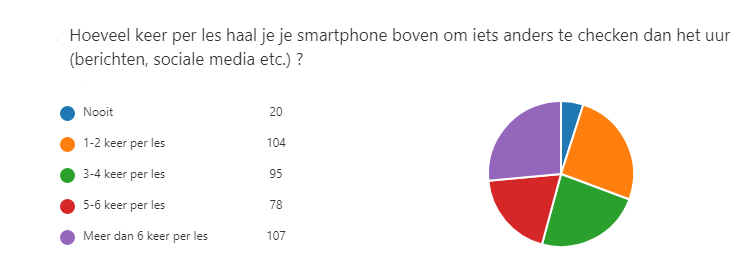
\includegraphics[width=\textwidth]
	{img/smartphone-social.png}
	\caption{Aantal keer dat studenten hun smartphone checken per les volgen de enquête (totaal: 404)}
	\label{fig:smartphone-social}
\end{figure}

Figuur \ref{fig:scatter1} toont ons het lineair verband tussen de variabelen "aantal keer per les checken van smartphone of laptop" en "gemiddeld cijfer op een examen (op 10)". Het is uit de grafiek al redelijk goed op te maken: er is weinig tot geen verband tussen deze 2 variabelen. Met een R-kwadraat-coëfficiënt van 0,0001 moeten we concluderen dat het aantal uur dat men achter een smartphone of laptop doorbrengt op een dag geen effect zal hebben op het uiteindelijk cijfer dat je behaalt. R-kwadraat-coëfficiënt is het kwadraat van de Pearson-correlatiecoëfficiënt, die aangeeft dat wanneer zijn waarde naar 1 neigt, de 2 variabelen een sterk lineair verband vertonen. 

\begin{figure}
	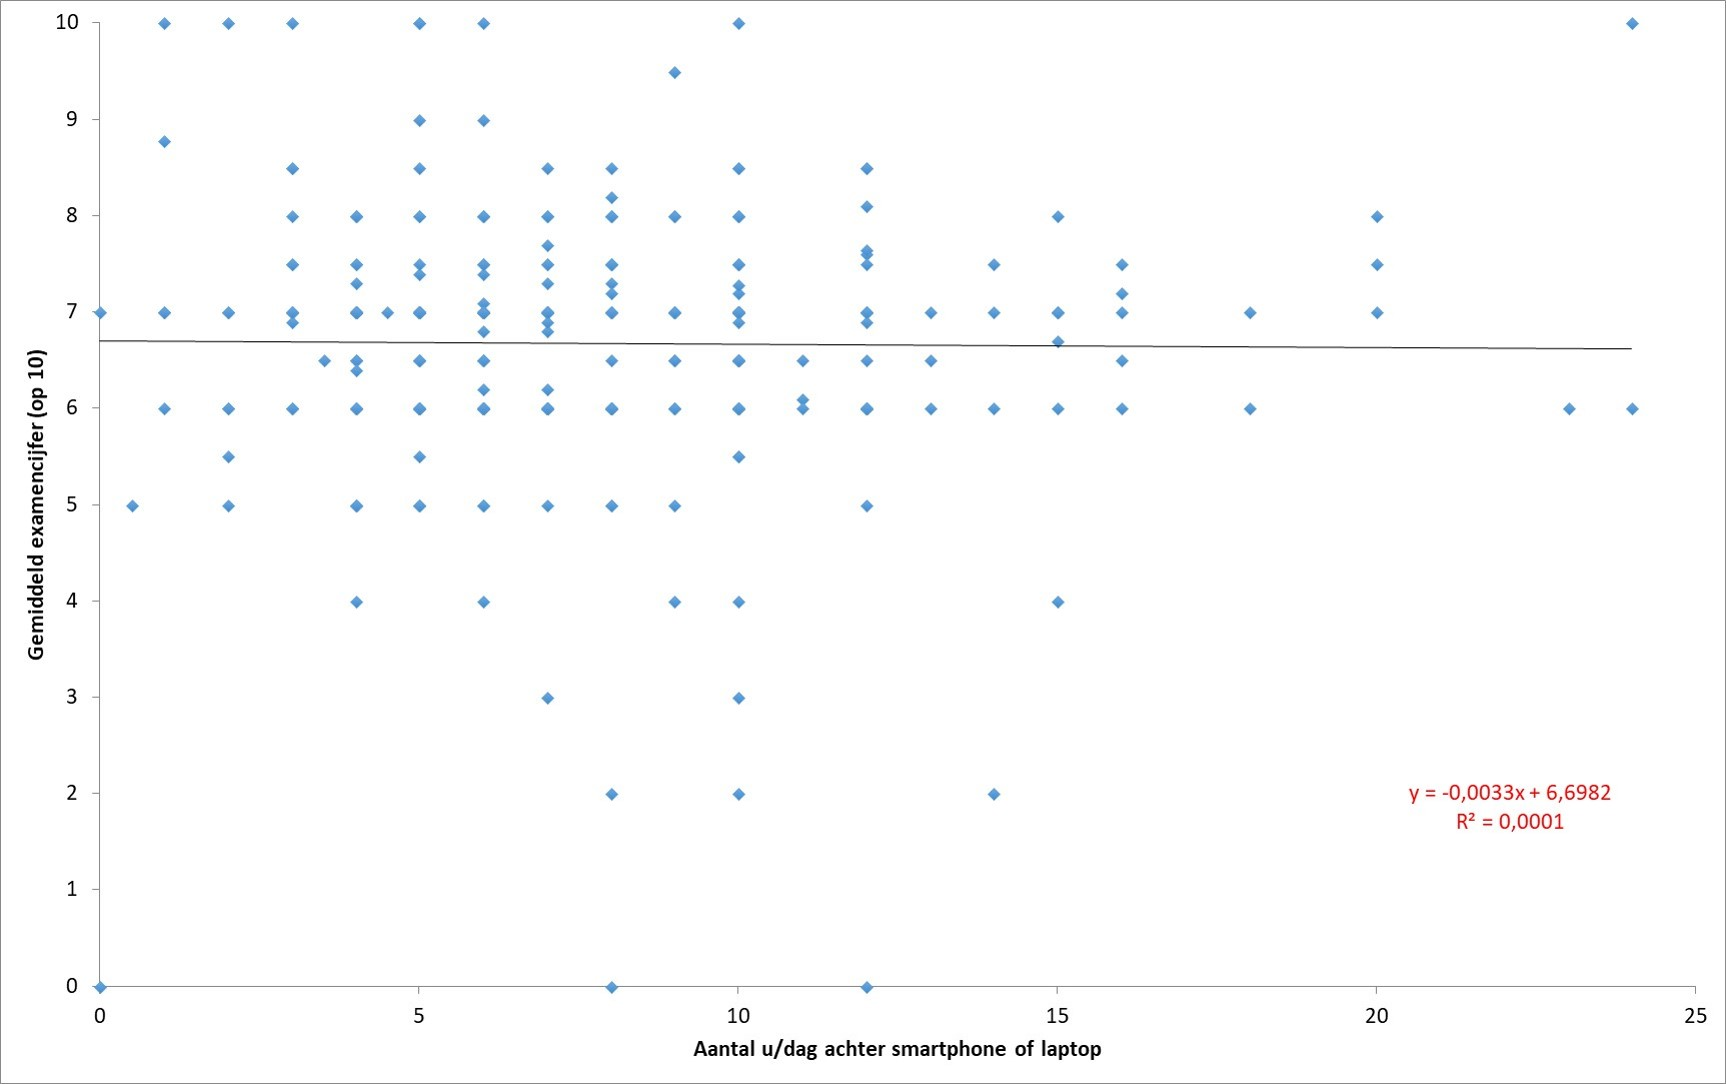
\includegraphics[width=\textwidth]
	{img/Scatter1.jpg}
	\caption{Lineair verband tussen aantal uur per dag achter smartphone of laptop en het gemiddeld cijfer op een examen (totaal: 404 studenten)}
	\label{fig:scatter1}
\end{figure}

Figuur \ref{fig:boxplot1} toont wel zeer positieve resultaten daarentegen. Hier hebben we voor elke categorie van aantal keer checken van smartphone tijdens de les een andere boxplot aangemaakt, die telkens de verschillende resultaten qua "gemiddeld examencijfer (op 10)" weergeeft. De uitschieters bij elke categorie zijn uitgefilterd uit alle boxplots. Deze grafiek toont aan dat studenten die nooit hun smartphone bekijken tijdens de les, op het einde van de rit ook gemiddeld een hoger cijfer halen dan studenten die wel hun smartphone regelmatig bekijken voor sociale media of berichten. En hoe meer je per les je smartphone bekijkt, hoe groter de kans ook is op het einde van het semester een lager gemiddeld cijfer te behalen voor je examens. Dit toont alleszins zeker aan dat hetgeen wat in de klas gebeurt met je smartphone, een effect heeft op je cijfer later.

\begin{figure}
	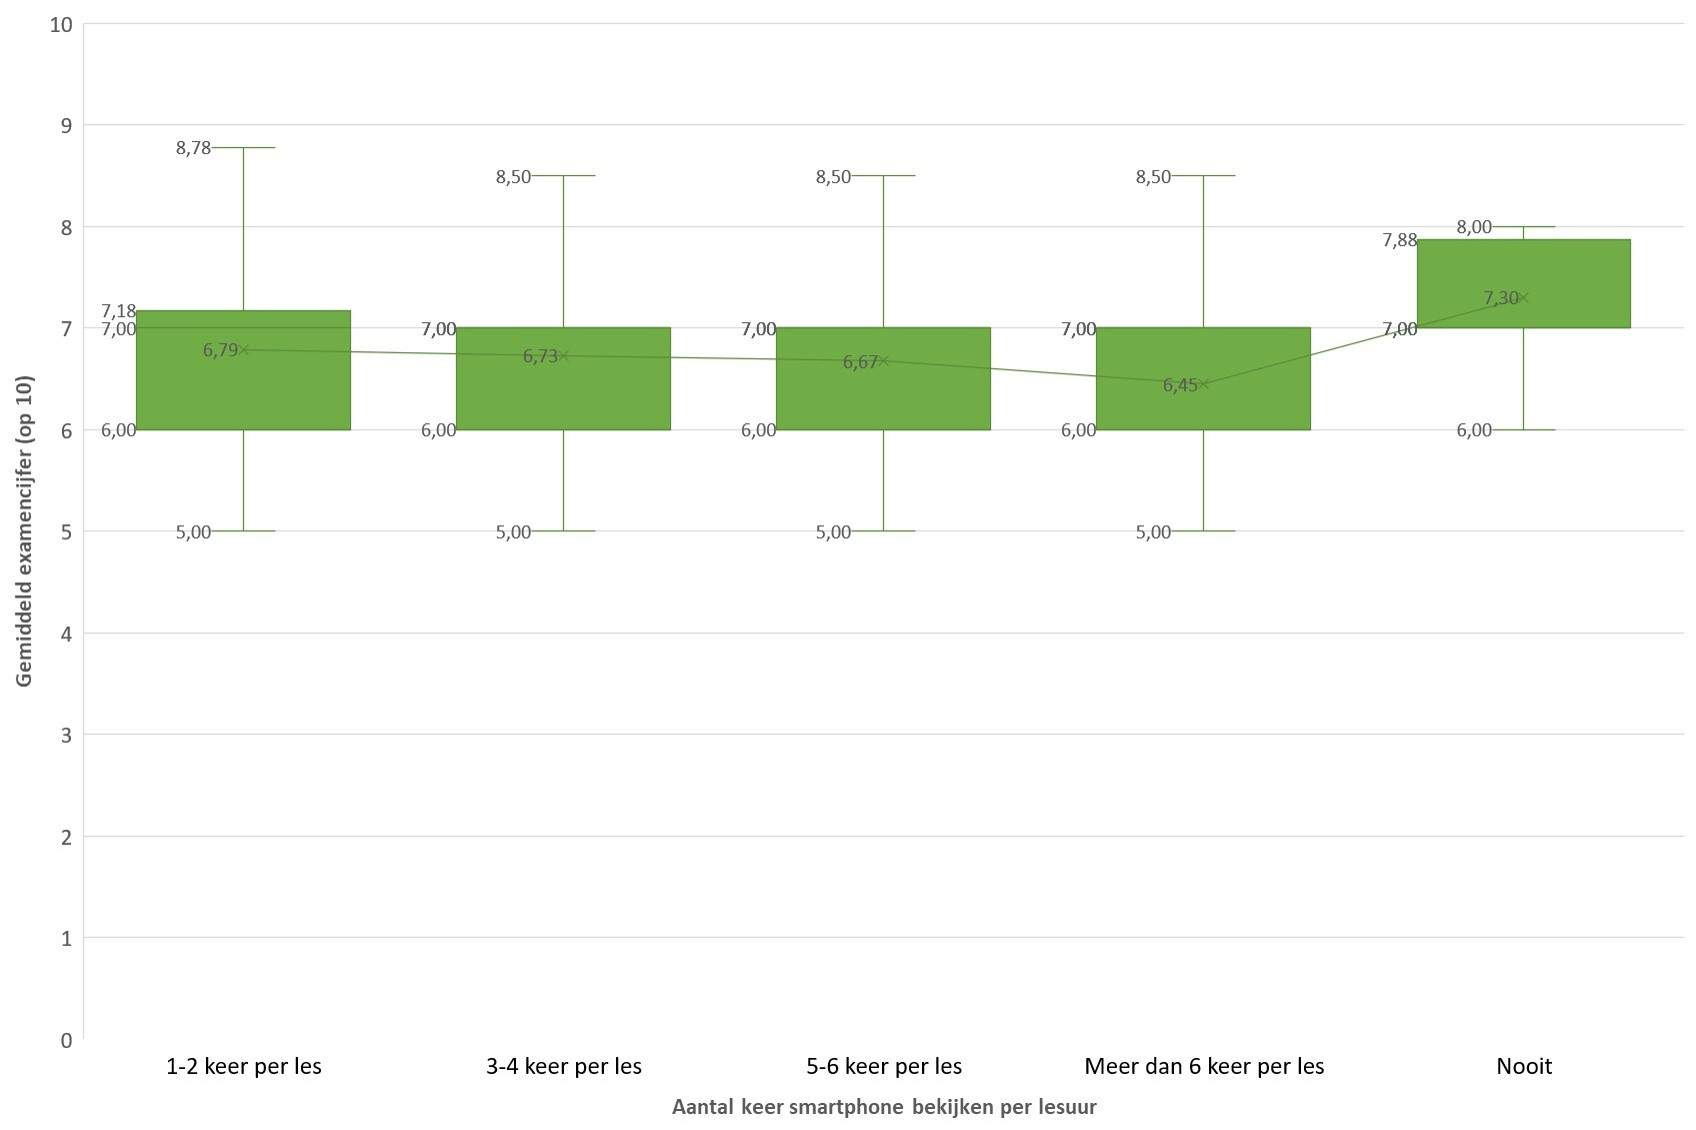
\includegraphics[width=\textwidth]
	{img/Boxplot1.jpg}
	\caption{Boxplots van gemiddeld studiecijfer voor elke categorie van 'aantal keer smartphone checken tijdens een lesuur' (totaal: 404 studenten)}
	\label{fig:boxplot1}
\end{figure}

Figuur \ref{fig:scatter2} maakt duidelijk dat er een zeer klein lineair verband is tussen het aantal vakken dat een student in 2de zit moet doorlopen en het aantal uur dat deze dagelijks spendeert achter zijn laptop of smartphone. Met een R-kwadraat-waarde van 0,007 mogen we niet stellen dat dit een heel sterk verband is, maar in tegenstelling tot het diagram in figuur \ref{fig:scatter1} kunnen we nu wel een lichte positieve rechte waarnemen.

\begin{figure}
	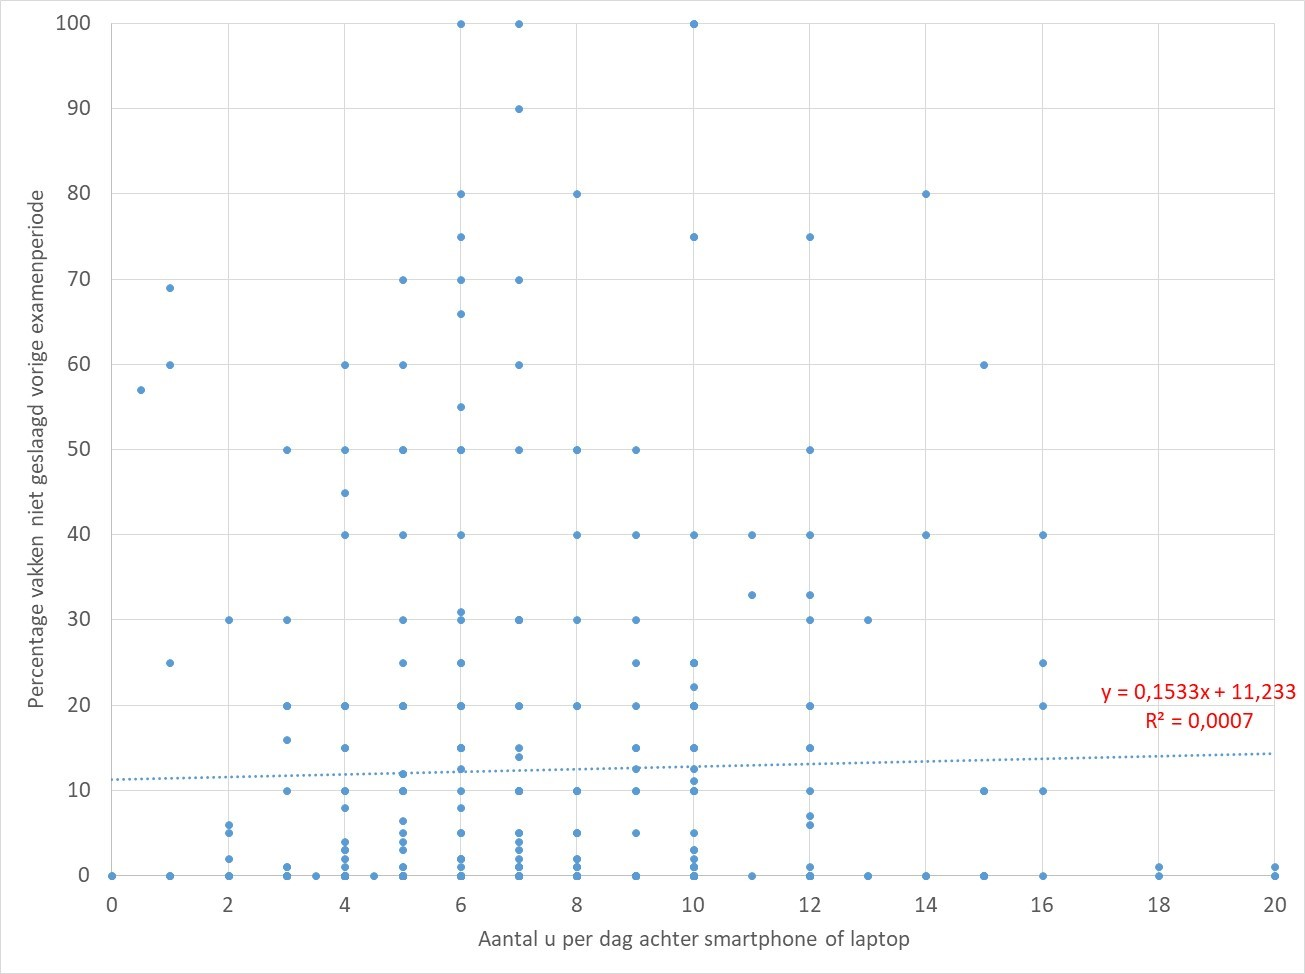
\includegraphics[width=\textwidth]
	{img/Scatter2.jpg}
	\caption{Lineair verband tussen het aantal uur per dag achter een smartphone of laptop en het percentage vakken waarvoor een student niet geslaagd was vorige examenperiode (totaal: 404 studenten)}
	\label{fig:scatter2}
\end{figure}

Figuur \ref{fig:boxplot2} toont dat studenten die nooit hun smartphone tijdens de les bovenhalen gemiddeld een lagere kans hebben op herexamens dan studenten die wel één of meerdere keren hun smartphone bovenhalen tijdens een theoretische les. Sowieso waren er veel van de ondervraagde studenten die de vorige examenperiode voor alles geslaagd waren, wat ook te zien is bij alle boxplots in deze grafiek (alle Q1 waarden zijn 0,00). Ondanks de zeer lage gemiddelde waarde bij studenten die 3 à 4 keer hun smartphone bovenhalen tijdens een lesuur, kan men toch afleiden uit de grafiek dat hoe meer je kijkt naar je smartphone, hoe (zeer miniem) de kans vergroot dat je een hoger percentage aan herkansingen zal moeten afleggen in de zomermaanden.

\begin{figure}
	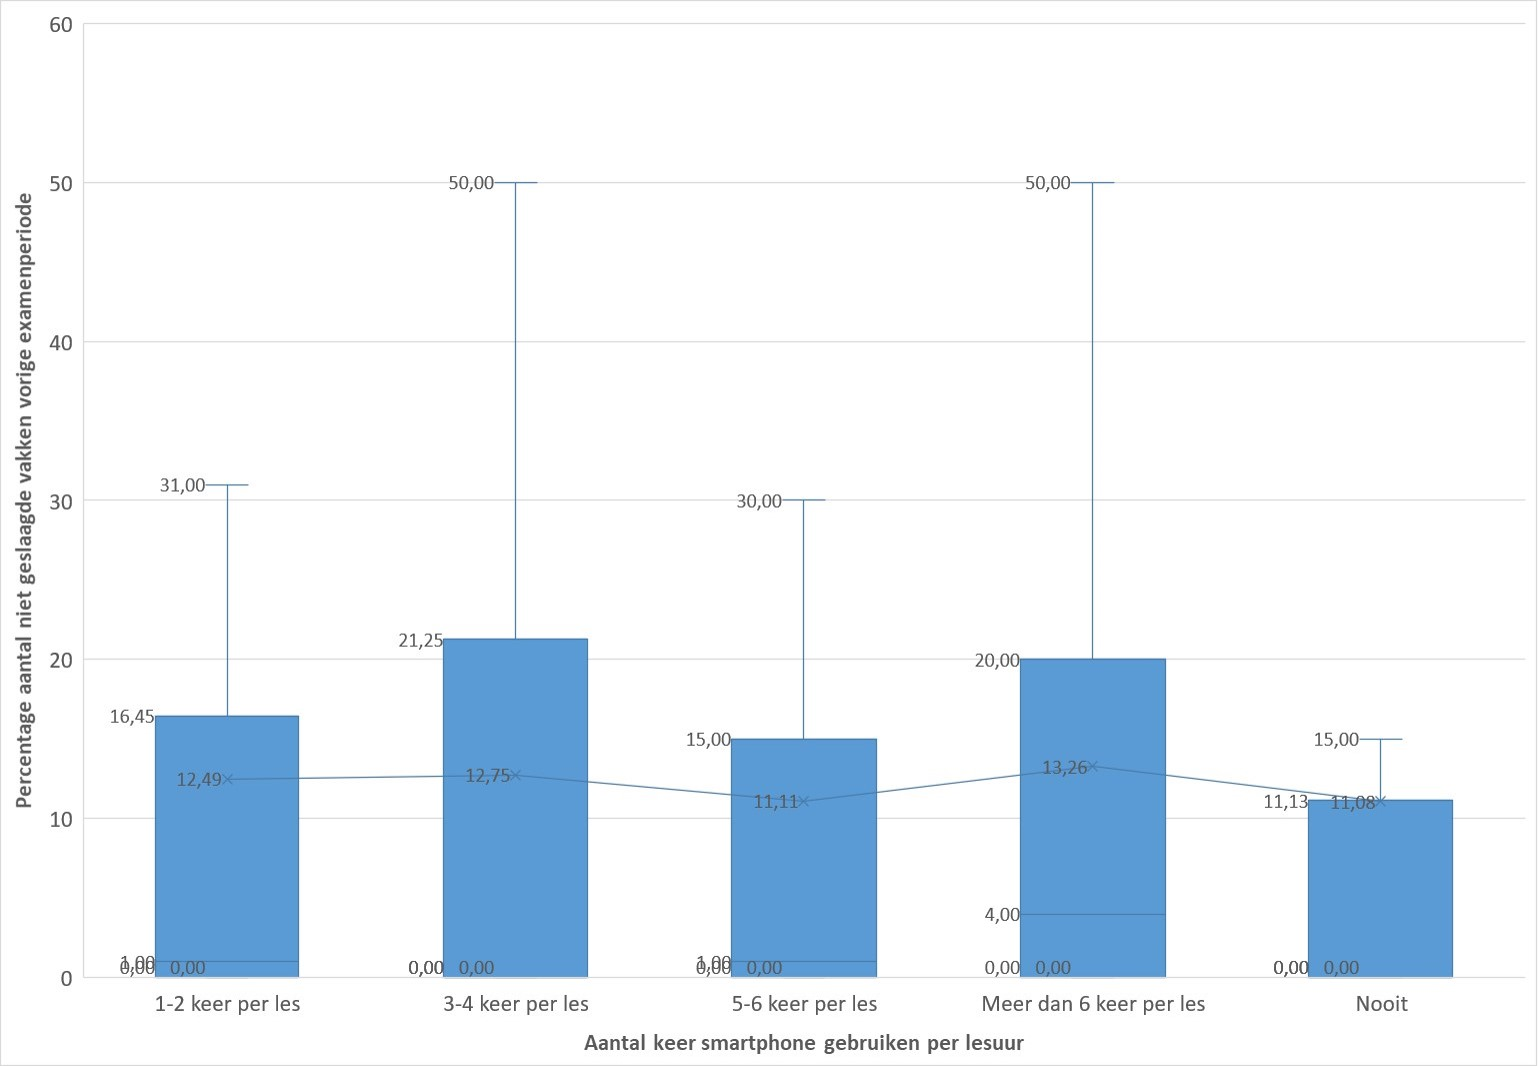
\includegraphics[width=\textwidth]
	{img/Boxplot2.jpg}
	\caption{Boxplots van het percentage vakken waarvoor student en onvoldoende haalde, verdeeld voor elke categorie van 'aantal keer smartphone checken tijdens een lesuur' (totaal: 404 studenten)}
	\label{fig:boxplot2}
\end{figure}

Deze resultaten tonen eigenlijk dat het niet uitmaakt wat je naast de les doet. Het is wat je in de les doet met je smartphone of laptop dat een miniem verschil kan maken of je net geslaagd bent voor een vak of niet, of dat het examenresultaat net dat tikkeltje beter is. Hoewel het allemaal kleine verschillen zijn, is er toch (zeker als je naar de boxplots kijkt) een trend te merken. Dat kleine stukje parate kennis dat je kan meenemen naar een examen wanneer je alle lessen hebt opgelet en geen of weinig aandacht hebt besteedt aan je smartphone of laptop, kan op het einde van de rit een groot verschil maken voor je examenresultaten.


\section{VRAAG 2: Heeft geslacht, relatiestatus of leeftijd van student een invloed op aantrekkingskracht die devices hebben op een student?}
\label{sec:geslacht-leeftijd}

Uit tabel \ref{results} kunnen we zien dat de grotere groep vrijgezellen terug te vinden is bij de personen die boven het gemiddelde scoren op vlak van devicegebruik. Ergens klinkt dit logisch: hoewel een student in relatie meer berichten stuurt met zijn of haar vriend(in), spendeert deze naar alle waarschijnlijkheid veel tijd met zijn of haar vriend(in). Vrijgezellen zijn mogelijks onzekerder over zichzelf of hebben net meer vrije tijd om bezig te zijn met gamen, sociale media en series te kijken op hun eentje. Een vrijgezel spendeert gemiddeld 7,69 uur achter zijn elektronische apparaten, waar een persoon die in een relatie is 7,30 uur met zijn dure apparaten doorbrengt. Een verschil van ongeveer 25 minuten per dag.

Uit dezelfde tabel kunnen we ook zien dat het aantal vrouwen in de 'laag gebruik'-groep zeer hoog is. Vrouwen spenderen dagelijks gemiddeld 7,14 uur achter een laptop of smartphone, waar mannen 8,09 uur spenderen achter een smartphone of laptop per dag, wat bijna een uur meer is. 
Vrouwen hebben wel meer een band met een smartphone tijdens de les dan jongens. Waar 52,56 procent van de vrouwen 5 keer of meer hun sociale status checken, of kijken of ze een nieuw berichtje hebben, gaan mannen hier minder vluchtig mee om. Bij hen kiest maar 36,47 procent ervoor om 5 keer of meer hun smartphone te checken tijdens de les. Mannen halen hun uur extra vooral dus uit hun tijd die ze spenderen achter hun laptop.

\begin{table}[]
	\centering
	\resizebox{\textwidth}{!}{%
	\begin{tabular}{llllll}
		& \multicolumn{5}{c}{\textbf{Geboortejaar}}                                                                 \\
		& \textbf{1995} & \textbf{1996} & \textbf{1997} & \textbf{1998}               & \textbf{1999}               \\
		\textbf{Aantal uur per dag achter laptop of smartphone}                                                                  & 7,33          & 8,18          & 6,72          & 7,72                        & 7,97                        \\
		\textbf{\begin{tabular}[c]{@{}l@{}}Percentage dat meer dan 5 keer\\ hun smartphone gebruikt tijdens de les\end{tabular}} & 43,47\%       & 47,54\%       & 52,13\%       & \multicolumn{1}{c}{43,84\%} & \multicolumn{1}{c}{52,08\%}
	\end{tabular}%
	}
	\caption{Correlatie tussen geboortejaar van teststudenten en hun dagelijks gebruik}
	\label{leeftijd}
\end{table}

Vervolgens kunnen we kijken naar de leeftijd van de student. In figuur \ref{leeftijd} kan u de verschillen per geboortejaar bekijken. Hieruit valt op dat deze resultaten zeer wisselvallig zijn. Hier valt niet echt een trend te spotten. Dit kan omwille van het aantal resultaten (mogelijks moet men meer dan 404 testresultaten verzamelen), maar het kan ook zijn dat sowieso studenten die in de jaren 90 geboren zijn gelijkaardig gedrag vertonen qua verslaving aan deze devices. Als we de lineaire samenhang onderzoeken tussen het jaar waarin een student geboren is en het aantal uur dat hij spendeert achter een smartphone of laptop per dag, dan is deze vrij weinig (Pearson-correlatiecoëfficient: 0,026). Er is dus weinig of geen verband tussen deze 2 variabelen.

\section{VRAAG 3: Is er een verschil in omgang met devices tussen Nederlandse en Vlaamse studenten?}
\label{sec:vlaanderen-nederland}

\begin{figure}
	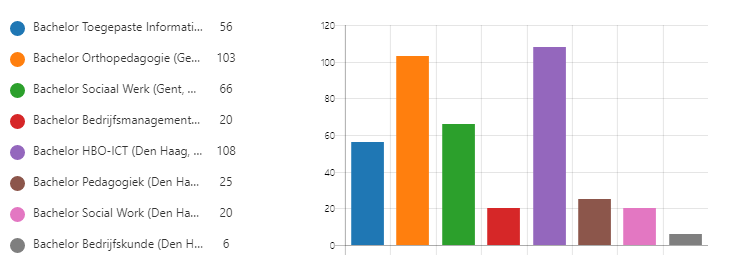
\includegraphics[width=\textwidth]
	{img/verdeling-enquete-richting.png}
	\caption{Verdeling van de studenten die geantwoord hebben op de enquête op basis van hun studierichting (totaal: 404)}
	\label{fig:verdeling-enquete-richting}
\end{figure}

In figuur \ref{fig:verdeling-enquete-richting} kan u zien hoeveel studenten van elke studierichting in België en Nederland de enquête hebben ingevuld. 

In tabel \ref{belg-nederlander} vindt u meer terug over de verschillen qua gebruik van elektronica tussen Vlaamse en Nederlandse studenten.

\begin{table}[]
	\centering
	\resizebox{\textwidth}{!}{%
		\begin{tabular}{lcc}
			& \multicolumn{2}{c}{\textbf{Hogeschool}}                                                                                                                           \\
			& \textbf{\begin{tabular}[c]{@{}c@{}}Haagse Hogeschool\\ Den Haag, Nederland\end{tabular}} & \textbf{\begin{tabular}[c]{@{}c@{}}HoGent\\ Gent, België\end{tabular}} \\
			\textbf{Aantal uur per dag achter laptop of smartphone}                                                                              & 8,35                                                                                     & 6,99                                                                   \\
			\textbf{\begin{tabular}[c]{@{}l@{}}Percentage studenten die meer dan 5 maal\\ hun smartphone gebruiken tijdens één les\end{tabular}} & 37,04\%                                                                                  & 51,65\%                                                                \\
			\textbf{Percentage smartphone mee in de les}                                                                                         & 98,77\%                                                                                  & 98,34\%                                                                \\
			\textbf{Percentage laptop mee in de les}                                                                                             & 85,80\%                                                                                  & 60,74\%                                                               
		\end{tabular}%
	}
	\caption{Verschillen in gebruik tussen België en Nederland}
	\label{belg-nederlander}
\end{table}

Hier moeten we rekening houden met het feit dat in België meer 'sociale' studenten zijn ondervraagd, waar in Nederland meer 'IT' studenten zijn ondervraagd. Maar zelfs als we hier rekening mee houden, kan men onmogelijk naast het feit kijken dat laptopgebruik tijdens de les meer ingeburgerd zit in Nederland dan in België. Waar maar 60,74 procent van de Vlaamse studenten hun laptop meebrengen naar de les, kiest wel 85,80 procent van de Nederlandse studenten ervoor om hun eigen laptop mee te brengen. Qua smartphones wisten we al het antwoord. We spreken bij smartphones enkel nog maar over enkelingen die geen mobieltje meebrengen naar school.

Het smartphonegebruik in België tijdens de les is bijna 15 procent hoger als in Nederland. Dit kan bijna volledig verklaard worden door het hoge aantal Vlaamse studenten uit de richting Orthopedagogie die deze enquête hebben ingevuld. Zoals u later kan lezen bij \ref{sec:sociale-it-richting}, wordt bij de sociale richtingen veel meer de smartphone bovengehaald tijdens de les dan bij de technische richtingen. 

\section{VRAAG 4: Wat denken studenten zelf over de invloed van smartphones op hun resultaten?}
\label{sec:invloed-resultaten}

\begin{figure}
	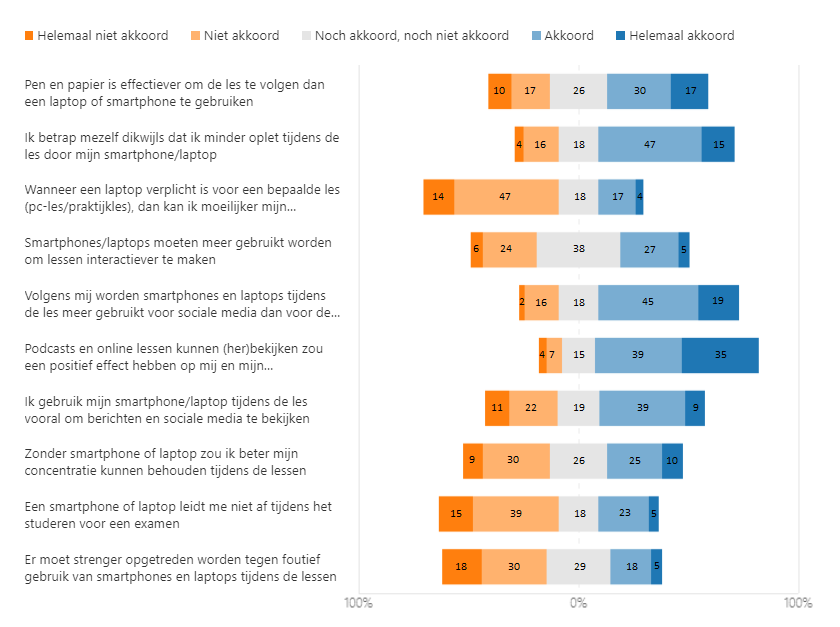
\includegraphics[width=\textwidth]
	{img/stellingen.png}
	\caption{Antwoorden van studenten op 10 stellingen over hun devices en de lessen (percentages afgerond naar gehele getallen)}
	\label{fig:stellingen}
\end{figure}

Studenten konden helemaal aan het einde van de enquête ook hun mening geven over 10 stellingen die verband houden met hun apparaten, school en cybergedrag. De resultaten hiervan kan u bekijken in figuur \ref{fig:stellingen}. 

De opvallendste resultaten zijn volgende:
\begin{itemize}
	\item Een grote groep van studenten (62,1 procent) is akkoord met de stelling dat smartphones en laptops tijdens de lessen ervoor zorgen dat ze minder gaan opletten tijdens de les. Ze betrappen zichzelf dat deze apparaten een vorm van afleiding bieden wanneer een les zich niet meer in hun interessegebied afspeelt.
	\item Iets meer dan 60 procent geeft ook aan dat wanneer laptops of smartphones toegelaten zijn voor het doeleinde van een les (m.a.w. PC- of praktijkles) dat studenten toch in staat zijn om hun aandacht volledig bij de les te houden. 
	\item Bijna 65 procent van de ondervraagde studenten denken, net zoals werd vooropgesteld in de inleiding van dit onderzoek, dat smartphones en laptops meer gebruikt worden voor sociale media te bekijken dan om mee de les te kunnen volgen. Maar 18 procent is het niet eens met deze stelling. 
	\item Podcasts en de mogelijkheid om online lessen te kunnen herbekijken zou volgens bijna 75 procent van de ondervraagden een positief effect hebben op de student. Of dit een positief effect is op het studieresultaat of de gemoedsrust van de student is hier niet duidelijk. Wel kan er mogelijks in de toekomst gekeken worden naar het belonen van studenten die naar de les komen en/of interesse tonen in wat de leerkracht te vertellen heeft.
	\item Verder kunnen we nog afleiden dat de helft van de studenten niet akkoord is met de stelling dat smartphones en laptops afleiden tijdens het studeren, dat iets meer dan de helft van de ondervraagden toegeeft hun elektronische devices te gebruiken voor berichtjes te sturen en sociale media te bekijken tijdens de les, en dat volgens een kleine meerderheid pen en papier een effectievere manier is om de les te kunnen volgen.
\end{itemize}

Een opmerking: achteraf bekeken heeft dit onderzoek de fout gemaakt om de optie 'Noch akkoord, noch niet akkoord' toe te voegen als mogelijke optie voor elke stelling. Hoewel deze 'middeloptie' meestal wordt aangeboden aan de invuller van een enquête zorgt deze ervoor dat bij sommige vragen deze categorie zo groot is dat het niet duidelijk is of er een meerderheid toch eerder akkoord gaat met een stelling of niet. Zo is bijvoorbeeld bij de vraag 'Smartphones/laptops moeten meer gebruikt worden om lessen interactiever te maken' deze groep zo groot (38,10 procent) dat het onmogelijk wordt om uit te maken of studenten eerder voor interactieve lessen zijn dan tegen. Het enigste bij deze stellingen dat men kan zeggen is dat de groep studenten zeer verdeeld is hierover.

\section{VRAAG 5: Is er verschil in gebruik van smartphones en in resultaten tussen studenten van sociale richting en studenten uit ICT-richting?}
\label{sec:sociale-it-richting}

Tabel \ref{it-social} toont de verschillen aan tussen enerzijds de studenten uit de richtingen HBO-ICT, Toegepaste Informatica, Bedrijfsmanagement en Bedrijfskunde (de 'IT-minded'-richtingen) en anderzijds de studenten uit de richtingen Social Work, Sociaal Werk, Pedagogiek en Orthopedagogie (de 'Social-minded'-richtingen).

Deze tabel toont zeer verschillende en soms tegenstrijdige resultaten. Bij de Vlaamse richtingen is het verschil tussen de IT-richtingen en de sociale richtingen gigantisch, waar in Nederland de resultaten dichter bij elkaar liggen. Algemeen kunnen we wel met zekerheid vaststellen dat IT-studies ook leiden tot een verhoogd aantal uur dat een student doorbrengt achter zijn pc, laptop of smartphone. Bijna 75 minuten per dag zit een IT- of Bedrijfsmanagement-student langer achter een scherm dan een student Orthopedagogie of Sociaal Werk. Het zijn vooral de studenten Toegepaste Informatica en de studenten Orthopedagogie, waar ook de meeste resultaten van kwamen in deze bevraging die deze getallen de hoogte in jagen. In België is het verschil zelfs bijna 2 uur per dag tussen sociale en it-minded studenten. Orthopedagogie steekt er op de Hogeschool Gent echt uit qua aantal uur. Dit is zeer tegenstrijdig met Nederland, waar ook zelfs in de sociale richtingen het aantal uur achter een laptop zeer hoog is, zelfs hoger dan bij een Nederlandse ICT of Bedrijfskunde-student. Vooral de HBO-ICT-studenten zijn zeer actief achter hun laptop en smartphone. De grote oorzaak hiervan is dat aan de Haagse Hogeschool bijna zo goed als niemand meer naar de les komt zonder een laptop. Rond de 85 procent van de Nederlandse studenten heeft een laptop mee naar de les, waar in Vlaanderen net geen 60 procent van de studenten hun laptop meebrengen naar de les.

Zeer opvallend, maar ook een verwachte uitkomst is dat het percentage studenten dat veel hun smartphone gebruiken tijdens de les hoger is in de sociale richtingen dan in de IT-richtingen. Net daar waar de nood aan laptops of smartphones het minst hoogst is, zal de student veel zijn smartphone gebruiken. Wat niet mag vergeten worden bij het bekijken van deze resultaten is dat studenten uit een IT-minded richting al vaak met een laptop voor hun neus zitten in de klas, en dus via deze weg vaak dezelfde dingen kunnen doen als op hun smartphone. De nood om de smartphone boven te halen tijdens de les is dus minder nodig in klassen waar laptops al een gewoonte zijn.

Men moet zeker niet vergeten rekening te houden met het feit dat voor de Nederlandse sociale richtingen er weinig respons was, en dat het aantal resultaten hier zeker te weinig is om te spreken over de representativiteit hiervan. Vooral het percentage over de IT-kennis van ouders springt hier onverklaarbaar de hoogte in.

\begin{table}[!h]
	\centering
	\resizebox{\textwidth}{!}{%
		\begin{tabular}{lcccccc}
			& \multicolumn{6}{c}{\textbf{Soort studierichting}}                                                                                                                                        \\
			& \multicolumn{3}{c}{\textbf{\begin{tabular}[c]{@{}c@{}}IT-Minded\\ richtingen\end{tabular}}} & \multicolumn{3}{c}{\textbf{\begin{tabular}[c]{@{}c@{}}Sociale \\ richtingen\end{tabular}}} \\
			& Algemeen                      & België                      & Nederland                     & Algemeen                     & België                      & Nederland                     \\
			\textbf{Aantal uur per dag achter laptop of smartphone}                                                                  & 8,24                          & 8,29                        & 8,20                          & 6,91                         & 6,39                        & 8,71                          \\
			\textbf{\begin{tabular}[c]{@{}l@{}}Percentage dat meer dan 5 keer\\ hun smartphone gebruikt tijdens de les\end{tabular}} & 32,11\%                       & 31,58\%                     & 32,46\%                       & 58,14\%                      & 61,08\%                     & 46.94\%                       \\
			\textbf{\begin{tabular}[c]{@{}l@{}}Percentage goede of uitstekende \\ IT-kennis van ouders\end{tabular}}                 & 23,68\%                       & 26,32\%                     & 22,93\%                       & 28,04\%                      & 22,49\%                     & 48,89\%                      
		\end{tabular}%
	}
	\caption{Resultaten verschil tussen IT-studies en sociale richtingen}
	\label{it-social}
\end{table}





